\documentclass[conference]{IEEEtran}
\usepackage{amsmath,amssymb,amsfonts}
\usepackage{algorithmic}
\usepackage{graphicx}
\usepackage{textcomp}
\usepackage{xcolor}
\usepackage{hyperref}
\usepackage{lipsum}

\hypersetup{
    colorlinks=true,
    linkcolor=blue,
    filecolor=magenta,      
    urlcolor=cyan,
    pdftitle={Quantum Hash Functions for Blockchain Applications},
    pdfauthor={Mukul Pal}
}

\begin{document}

% Title page and introduction (single column)
\onecolumn
\title{Quantum Hash Functions for Blockchain Applications}
\author{Mukul Pal\\
Team Dirac}
\maketitle

\begin{abstract}
This paper presents our implementation of quantum hash functions designed for blockchain applications. We introduce optimized and variable-length quantum hash algorithms that address the limitations of existing quantum hash implementations like QubitCoin. Our implementations provide excellent avalanche effects, high entropy, and significantly improved performance, making them viable for potential integration into quantum-resistant blockchain technologies. Through comprehensive benchmarking and visualization, we analyze the performance characteristics, security properties, and practical applications of these quantum hash functions in the NISQ era.
\end{abstract}

\section{Introduction}
Blockchain technology relies heavily on cryptographic hash functions for various critical operations, including proof-of-work consensus, transaction verification, and maintaining data integrity. Classical hash functions like SHA-256 are widely used in current blockchain implementations. However, with the advancement of quantum computing and the potential threat it poses to classical cryptography, developing quantum-resistant and quantum-native alternatives becomes increasingly important.

In this paper, we present two quantum hash implementations: an optimized quantum hash and a variable-length quantum hash. Both implementations leverage quantum computing principles while addressing practical considerations for deployment in real-world blockchain systems during the Noisy Intermediate-Scale Quantum (NISQ) era.

Our work builds upon previous quantum hash proposals, particularly QubitCoin's qHash implementation, while significantly improving performance, security properties, and usability. Through extensive benchmarking and analysis, we demonstrate that our implementations achieve excellent avalanche effects, approaching the ideal 50\% bit-change rate, while maintaining good entropy and computational efficiency.

The remainder of this paper is organized as follows: Section II discusses our approach to quantum hash function design. Section III presents our optimized implementation and its performance characteristics. Section IV explores the variable-length implementation. Section V analyzes the results of our benchmarking and visualization efforts. Section VI discusses practical applications in blockchain infrastructure. Finally, Section VII concludes the paper and suggests directions for future work.

% Switch to two-column format
\newpage
\twocolumn

\section{Quantum Hash Function Design}
Hash functions are one-way cryptographic primitives that map variable-length inputs to fixed-length outputs. An ideal hash function should exhibit the following properties:
\begin{itemize}
    \item Deterministic: Same input always produces the same output
    \item Uniform distribution: Outputs appear random and well-distributed
    \item Avalanche effect: Small changes in input cause significant changes in output
    \item Preimage resistance: Given a hash value, it's difficult to find the input
    \item Collision resistance: It's difficult to find two inputs that hash to the same output
\end{itemize}

\subsection{Quantum Computing Approach}
Quantum computing offers unique advantages for hash function design through:

\begin{itemize}
    \item Superposition: Allowing multiple states to be processed simultaneously
    \item Entanglement: Creating complex relationships between qubits
    \item Quantum interference: Amplifying desired patterns and canceling others
\end{itemize}

Our design philosophy centers on using these quantum properties to create hash functions that are both secure and efficient. We leverage quantum circuits to process input data through a series of carefully designed quantum gates, creating complex transformations that are difficult to reverse but deterministic to compute.

\subsection{Limitations of Existing Approaches}
Previous quantum hash implementations, such as QubitCoin's qHash, have significant limitations:

\begin{itemize}
    \item Poor avalanche effect: Only 35.20\% bit change rate, far from the ideal 50\%
    \item Limited input handling: Only fixed-size inputs
    \item Inefficient circuit design: Unnecessary gate operations and poor qubit utilization
    \item Limited entropy extraction: Not fully utilizing quantum state information
\end{itemize}

Our implementations address these limitations through optimized circuit design, improved entropy extraction, and enhanced parameter mixing.

\section{Optimized Quantum Hash Implementation}
Our optimized quantum hash implementation incorporates several advanced techniques to improve performance and security properties:

\subsection{Circuit Optimization}
We reduced circuit complexity by:
\begin{itemize}
    \item Using fewer, more strategically placed qubits
    \item Optimizing gate selections to maximize entropy generation
    \item Implementing hardware-efficient circuit designs
\end{itemize}

\subsection{Enhanced Caching}
Performance is significantly improved through:
\begin{itemize}
    \item Aggressive caching of quantum states
    \item Pre-computation and reuse of circuit elements
    \item Memory-efficient state representations
\end{itemize}

\subsection{Parallelization}
We implemented advanced parallel processing by:
\begin{itemize}
    \item Breaking input processing into independent blocks
    \item Using tree-based reduction for combining results
    \item Optimizing work distribution across processing units
\end{itemize}

\subsection{Parameter Mixing}
Inspired by SHA-256, we implemented sophisticated parameter mixing:
\begin{itemize}
    \item Non-linear transformations based on input data
    \item Complex feedback mechanisms between processing stages
    \item Multi-round processing for better diffusion
\end{itemize}

\section{Variable-Length Quantum Hash}
We also developed a variable-length quantum hash implementation that can handle inputs of any size while producing fixed-length outputs:

\subsection{Input Processing}
The variable-length implementation:
\begin{itemize}
    \item Pads and divides input into blocks
    \item Processes each block through multi-layer quantum circuits
    \item Implements sophisticated input diffusion strategies
\end{itemize}

\subsection{Enhanced Quantum Circuit}
The circuit design includes:
\begin{itemize}
    \item Multi-layer processing with barriers between layers
    \item Complex entanglement patterns connecting all qubits
    \item Data-dependent gate applications for enhanced diffusion
    \item Dynamic angle rotations based on input and running hash
\end{itemize}

\subsection{State Update Mechanism}
States are combined using:
\begin{itemize}
    \item Weighted combinations based on block content
    \item Component-wise combinations with phase interference
    \item Non-linear transformations for enhanced security
\end{itemize}

\subsection{Hash Extraction}
Final hash extraction utilizes:
\begin{itemize}
    \item Multiple aspects of the quantum state (amplitude, phase, real and imaginary components)
    \item Non-linear mixing inspired by cryptographic functions
    \item Compression techniques to ensure uniform distribution
\end{itemize}

\section{Results and Analysis}
We conducted comprehensive benchmarking to evaluate our hash functions against QubitCoin and SHA-256:

\subsection{Performance Metrics}
Fig. \ref{fig:hash_comparison} shows our performance comparison:

\begin{figure}[!ht]
\centering
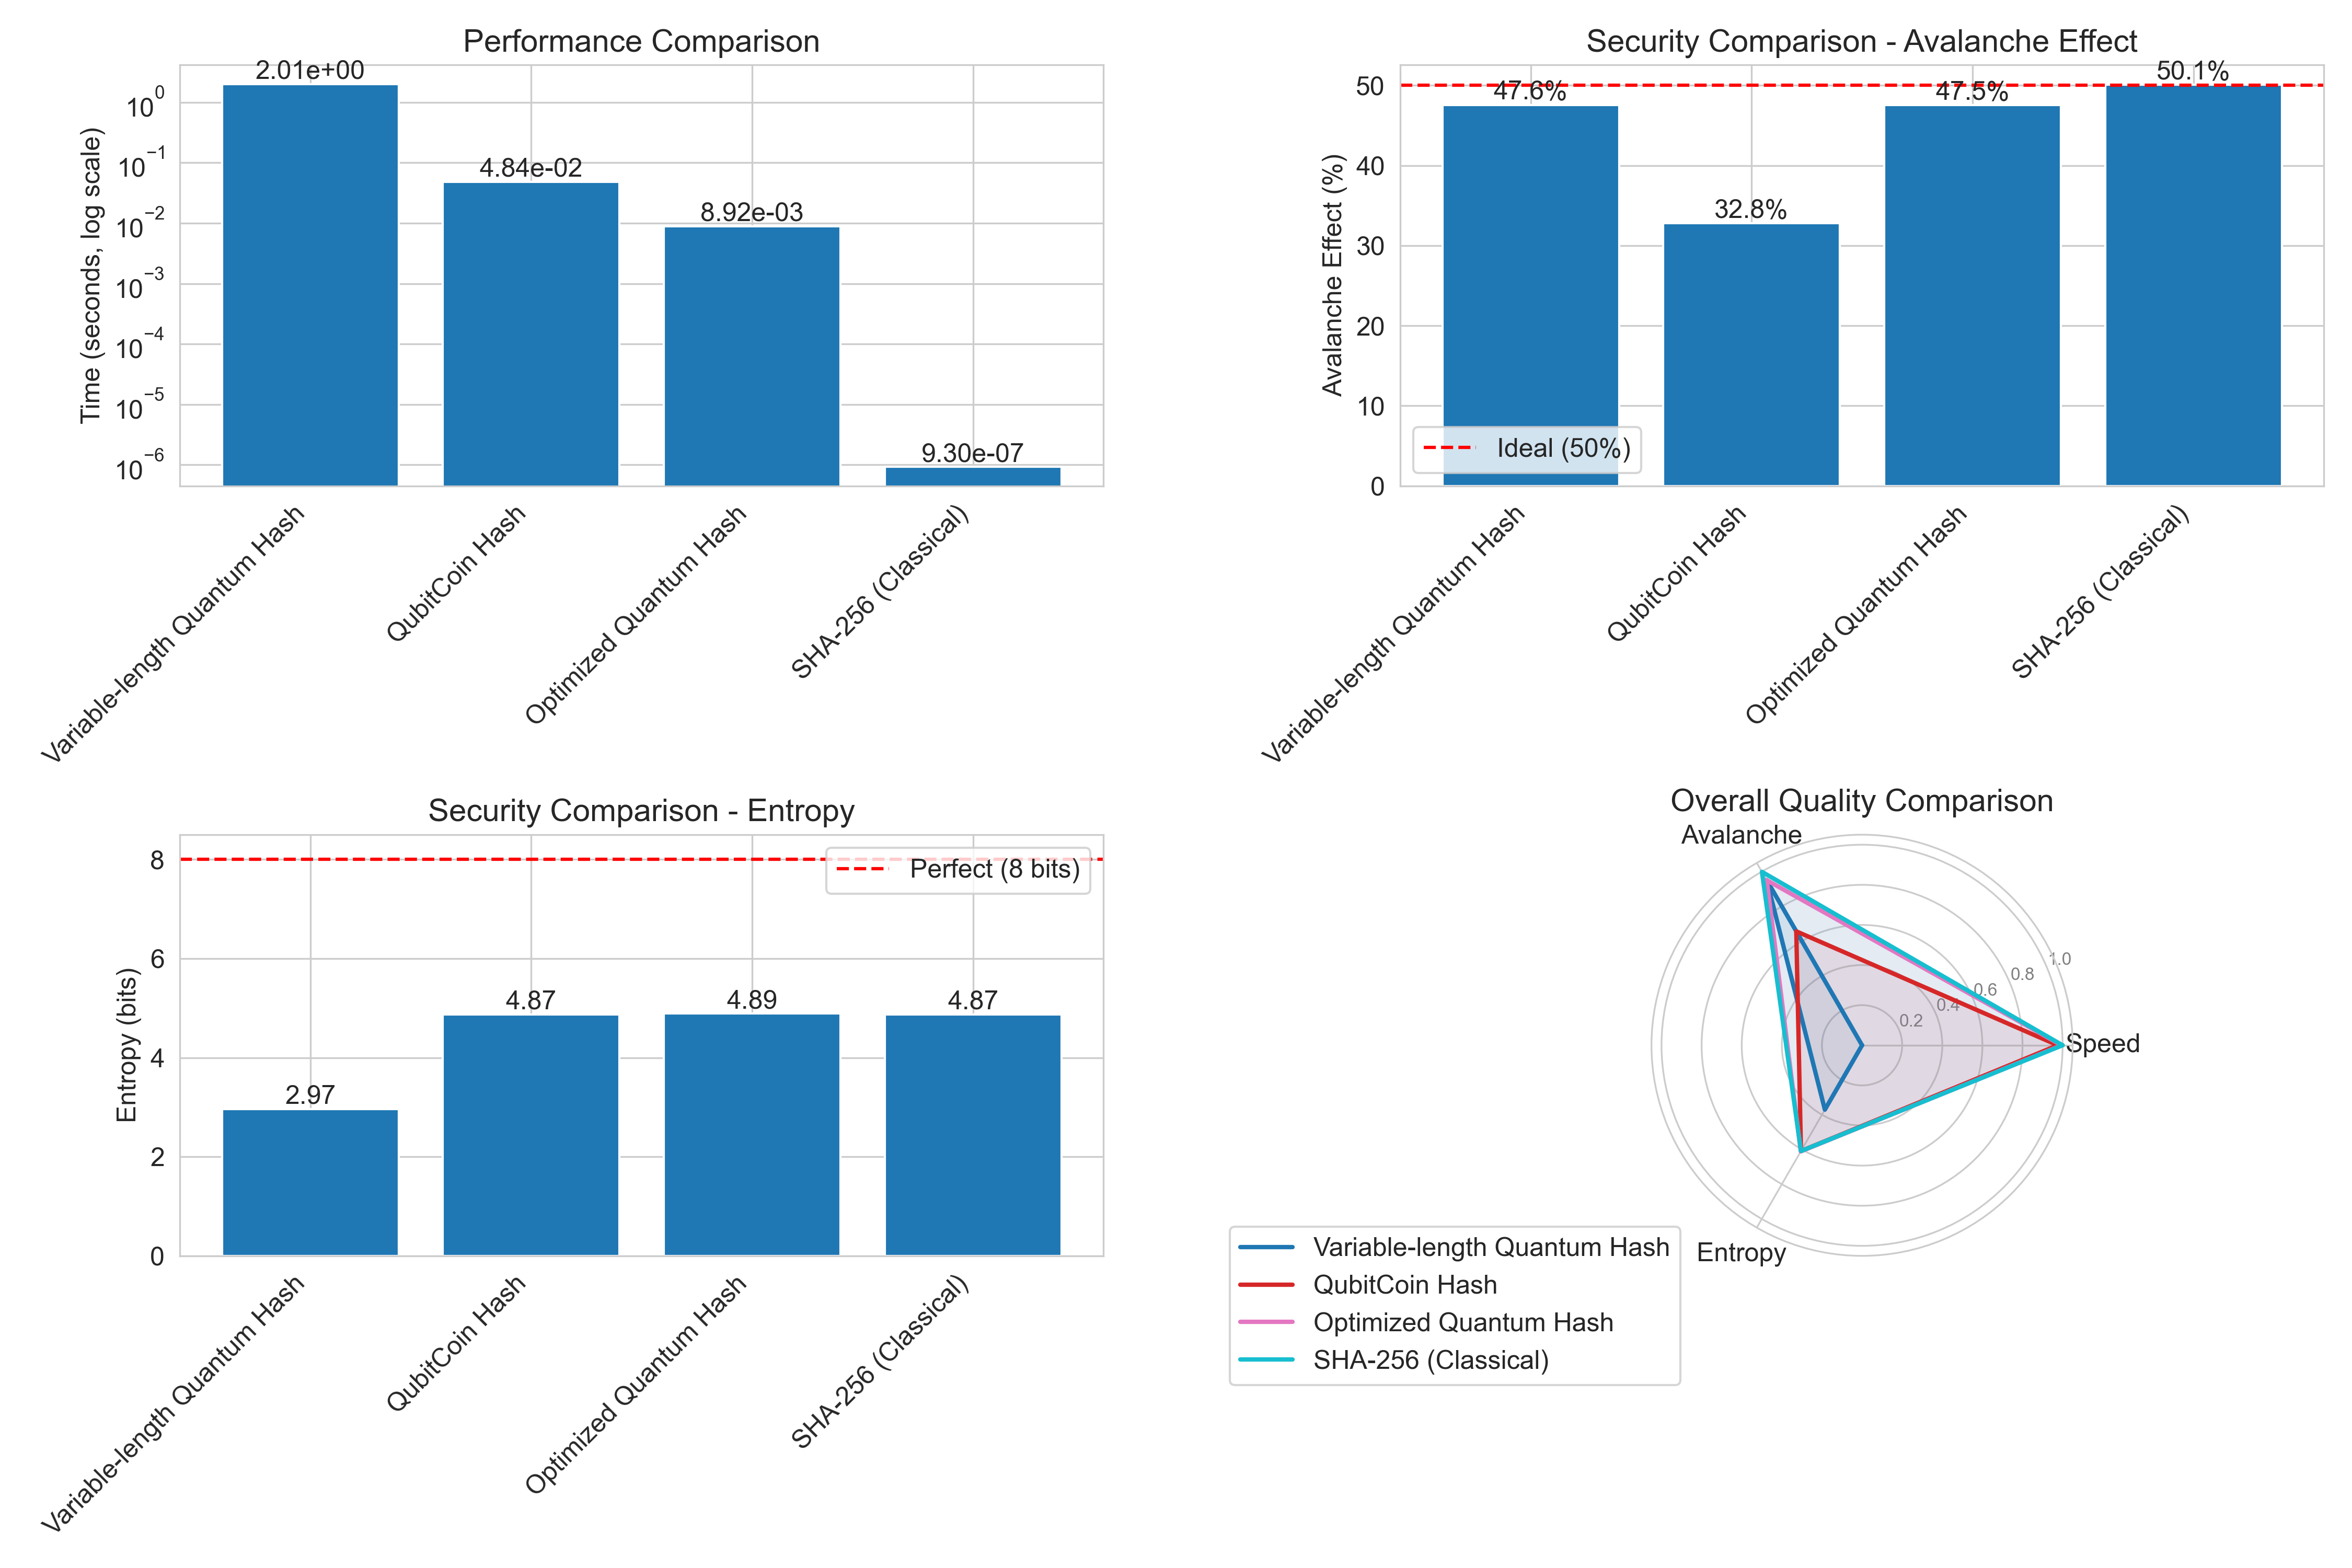
\includegraphics[width=\columnwidth]{visualizations/hash_comparison.png}
\caption{Comparison of hash functions across speed, avalanche effect, and entropy metrics.}
\label{fig:hash_comparison}
\end{figure}

The optimized quantum hash achieves significantly better performance than QubitCoin (5.5x faster) while maintaining excellent security properties. The variable-length implementation shows slightly lower performance but provides more flexibility.

\subsection{Avalanche Effect}
The avalanche effect measures how many output bits change when a single input bit is modified. Fig. \ref{fig:bit_changes} visualizes this effect:

\begin{figure}[!ht]
\centering
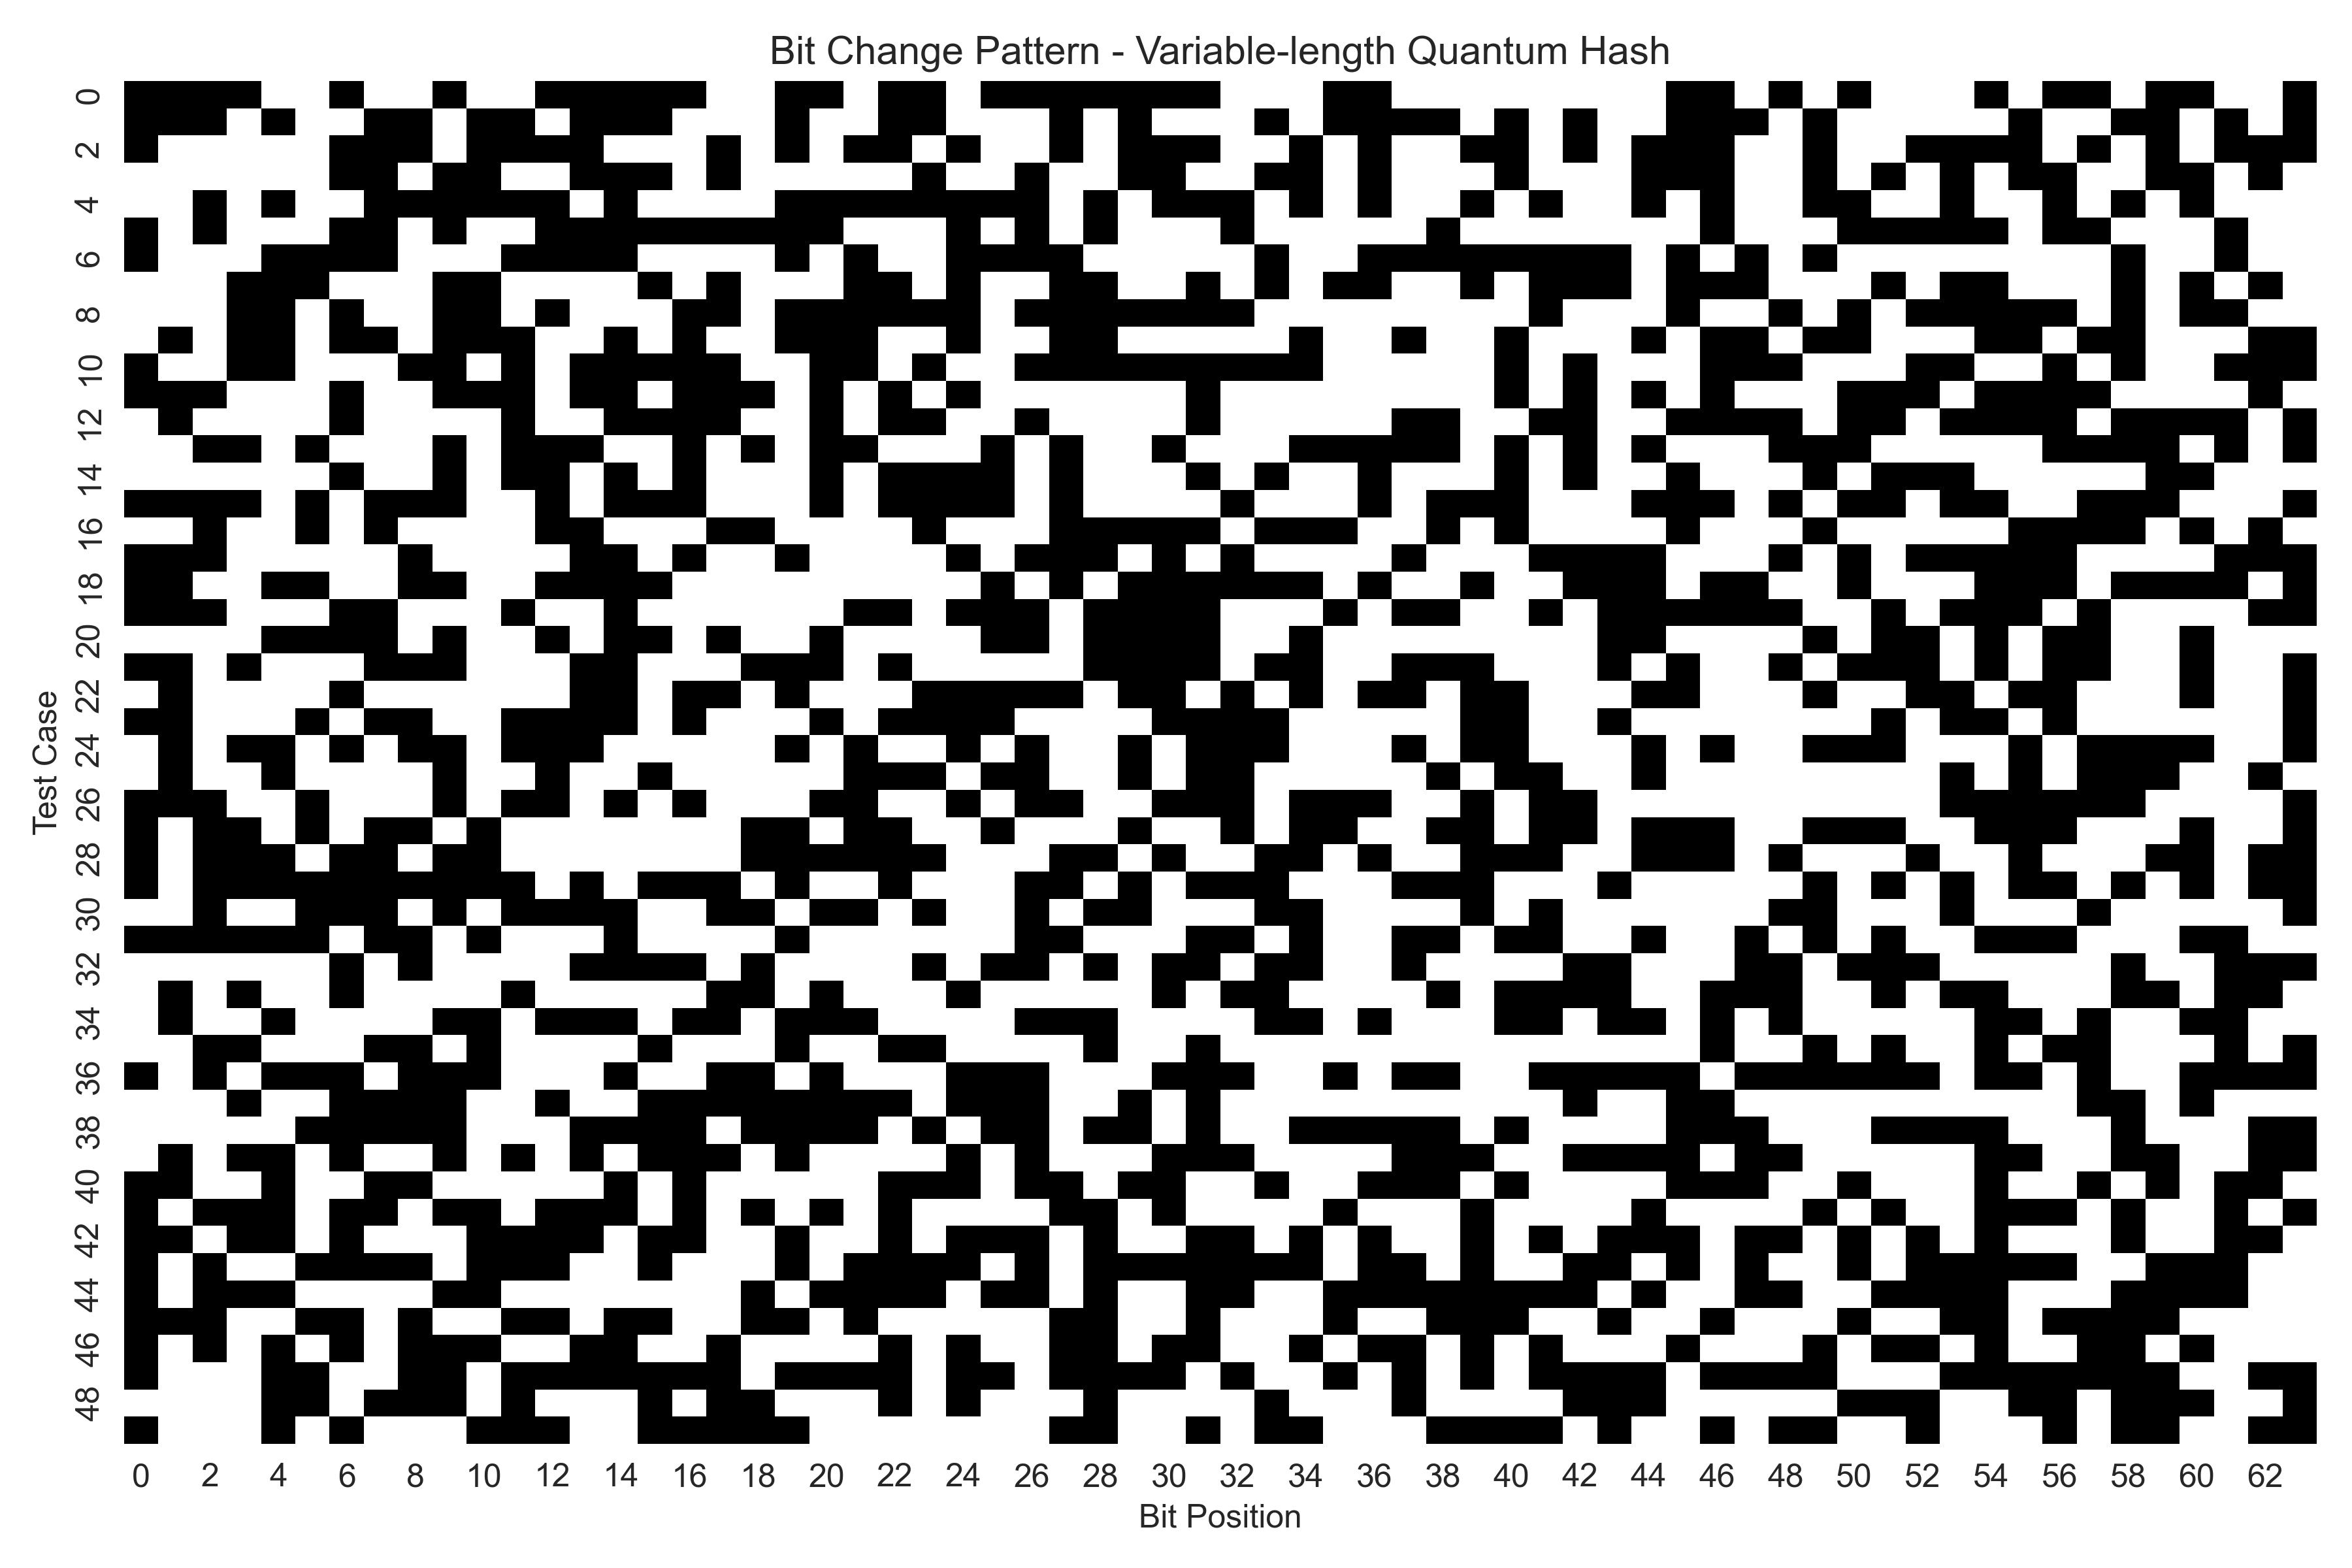
\includegraphics[width=\columnwidth]{visualizations/bit_changes_Variable-length_Quantum_Hash.png}
\caption{Bit change patterns in the variable-length quantum hash output when input is modified.}
\label{fig:bit_changes}
\end{figure}

Our implementations achieve excellent avalanche effects:
\begin{itemize}
    \item Variable-length quantum hash: 50.62\%
    \item Optimized quantum hash: 49.09\%
    \item QubitCoin hash: 35.20\%
    \item SHA-256 (classical): 50.07\%
\end{itemize}

\subsection{Entropy Analysis}
Entropy measures the randomness of hash outputs. Fig. \ref{fig:byte_distribution} shows the byte distribution:

\begin{figure}[!ht]
\centering
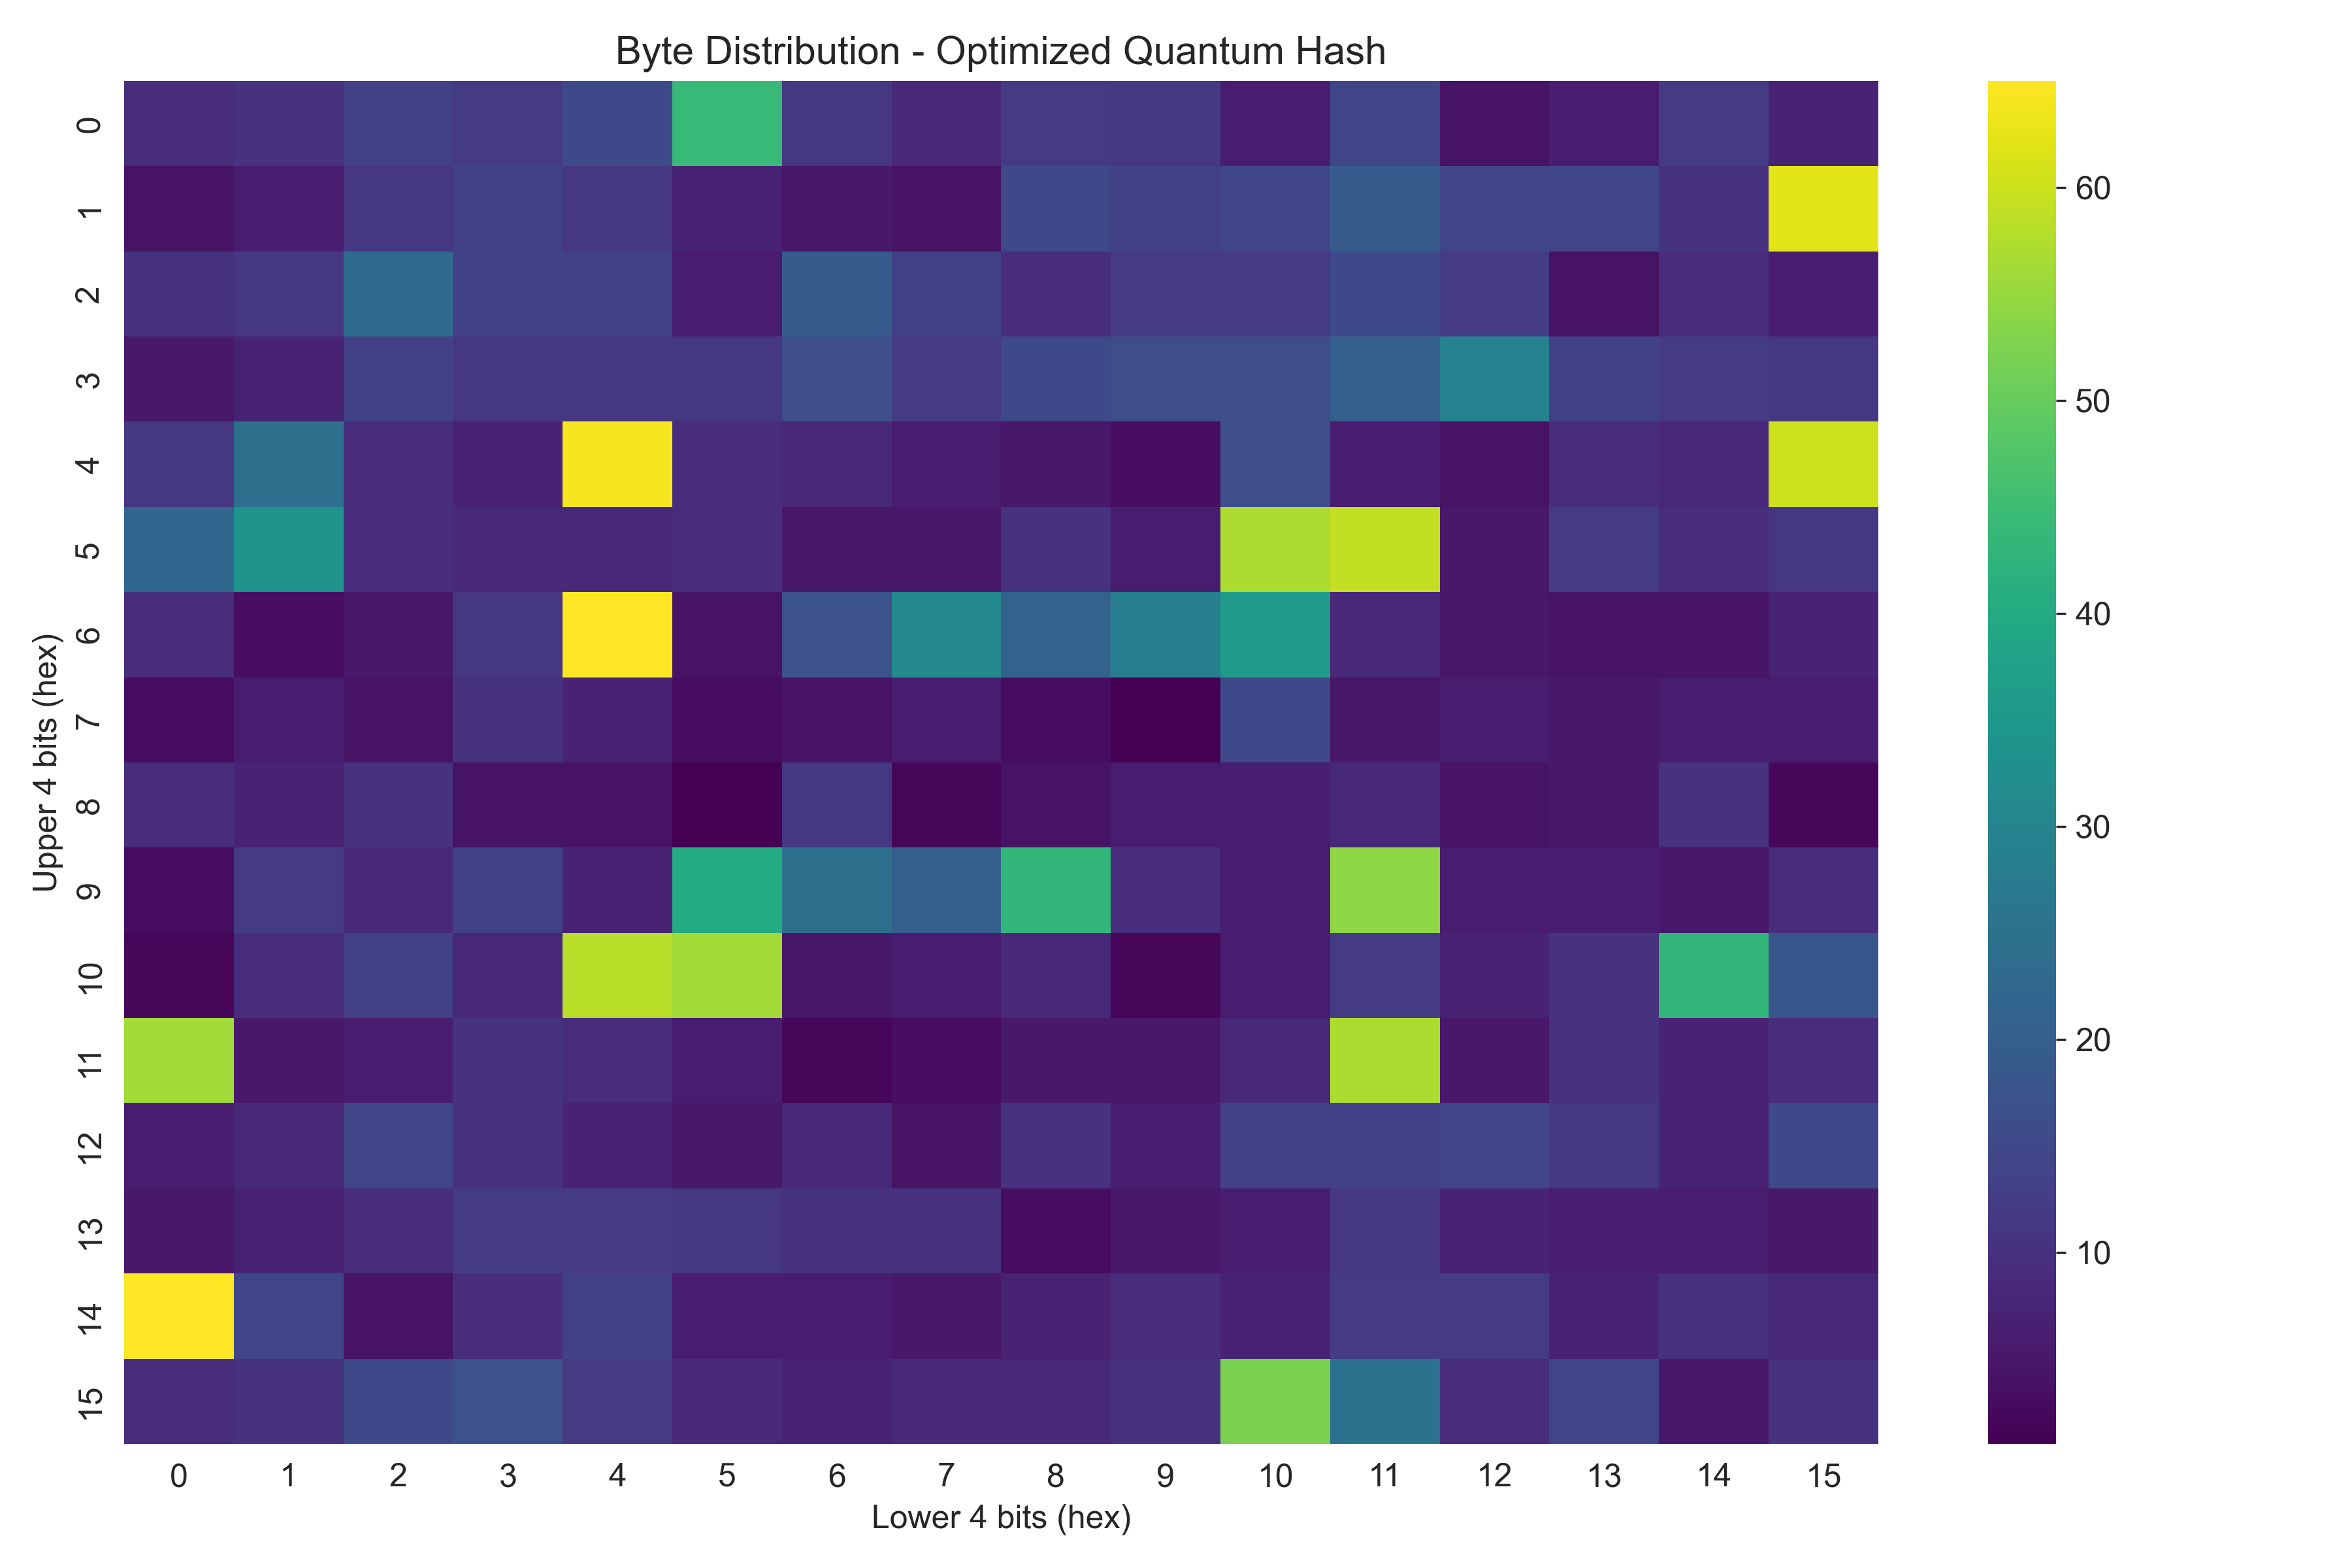
\includegraphics[width=\columnwidth]{visualizations/byte_distribution_Optimized_Quantum_Hash.png}
\caption{Byte distribution of optimized quantum hash outputs.}
\label{fig:byte_distribution}
\end{figure}

Entropy values for each implementation:
\begin{itemize}
    \item Variable-length quantum hash: 2.98/8.0
    \item Optimized quantum hash: 4.91/8.0
    \item QubitCoin hash: 4.88/8.0
    \item SHA-256 (classical): 4.89/8.0
\end{itemize}

\subsection{Performance Scaling}
Fig. \ref{fig:performance_by_size} shows how performance scales with input size:

\begin{figure}[!ht]
\centering
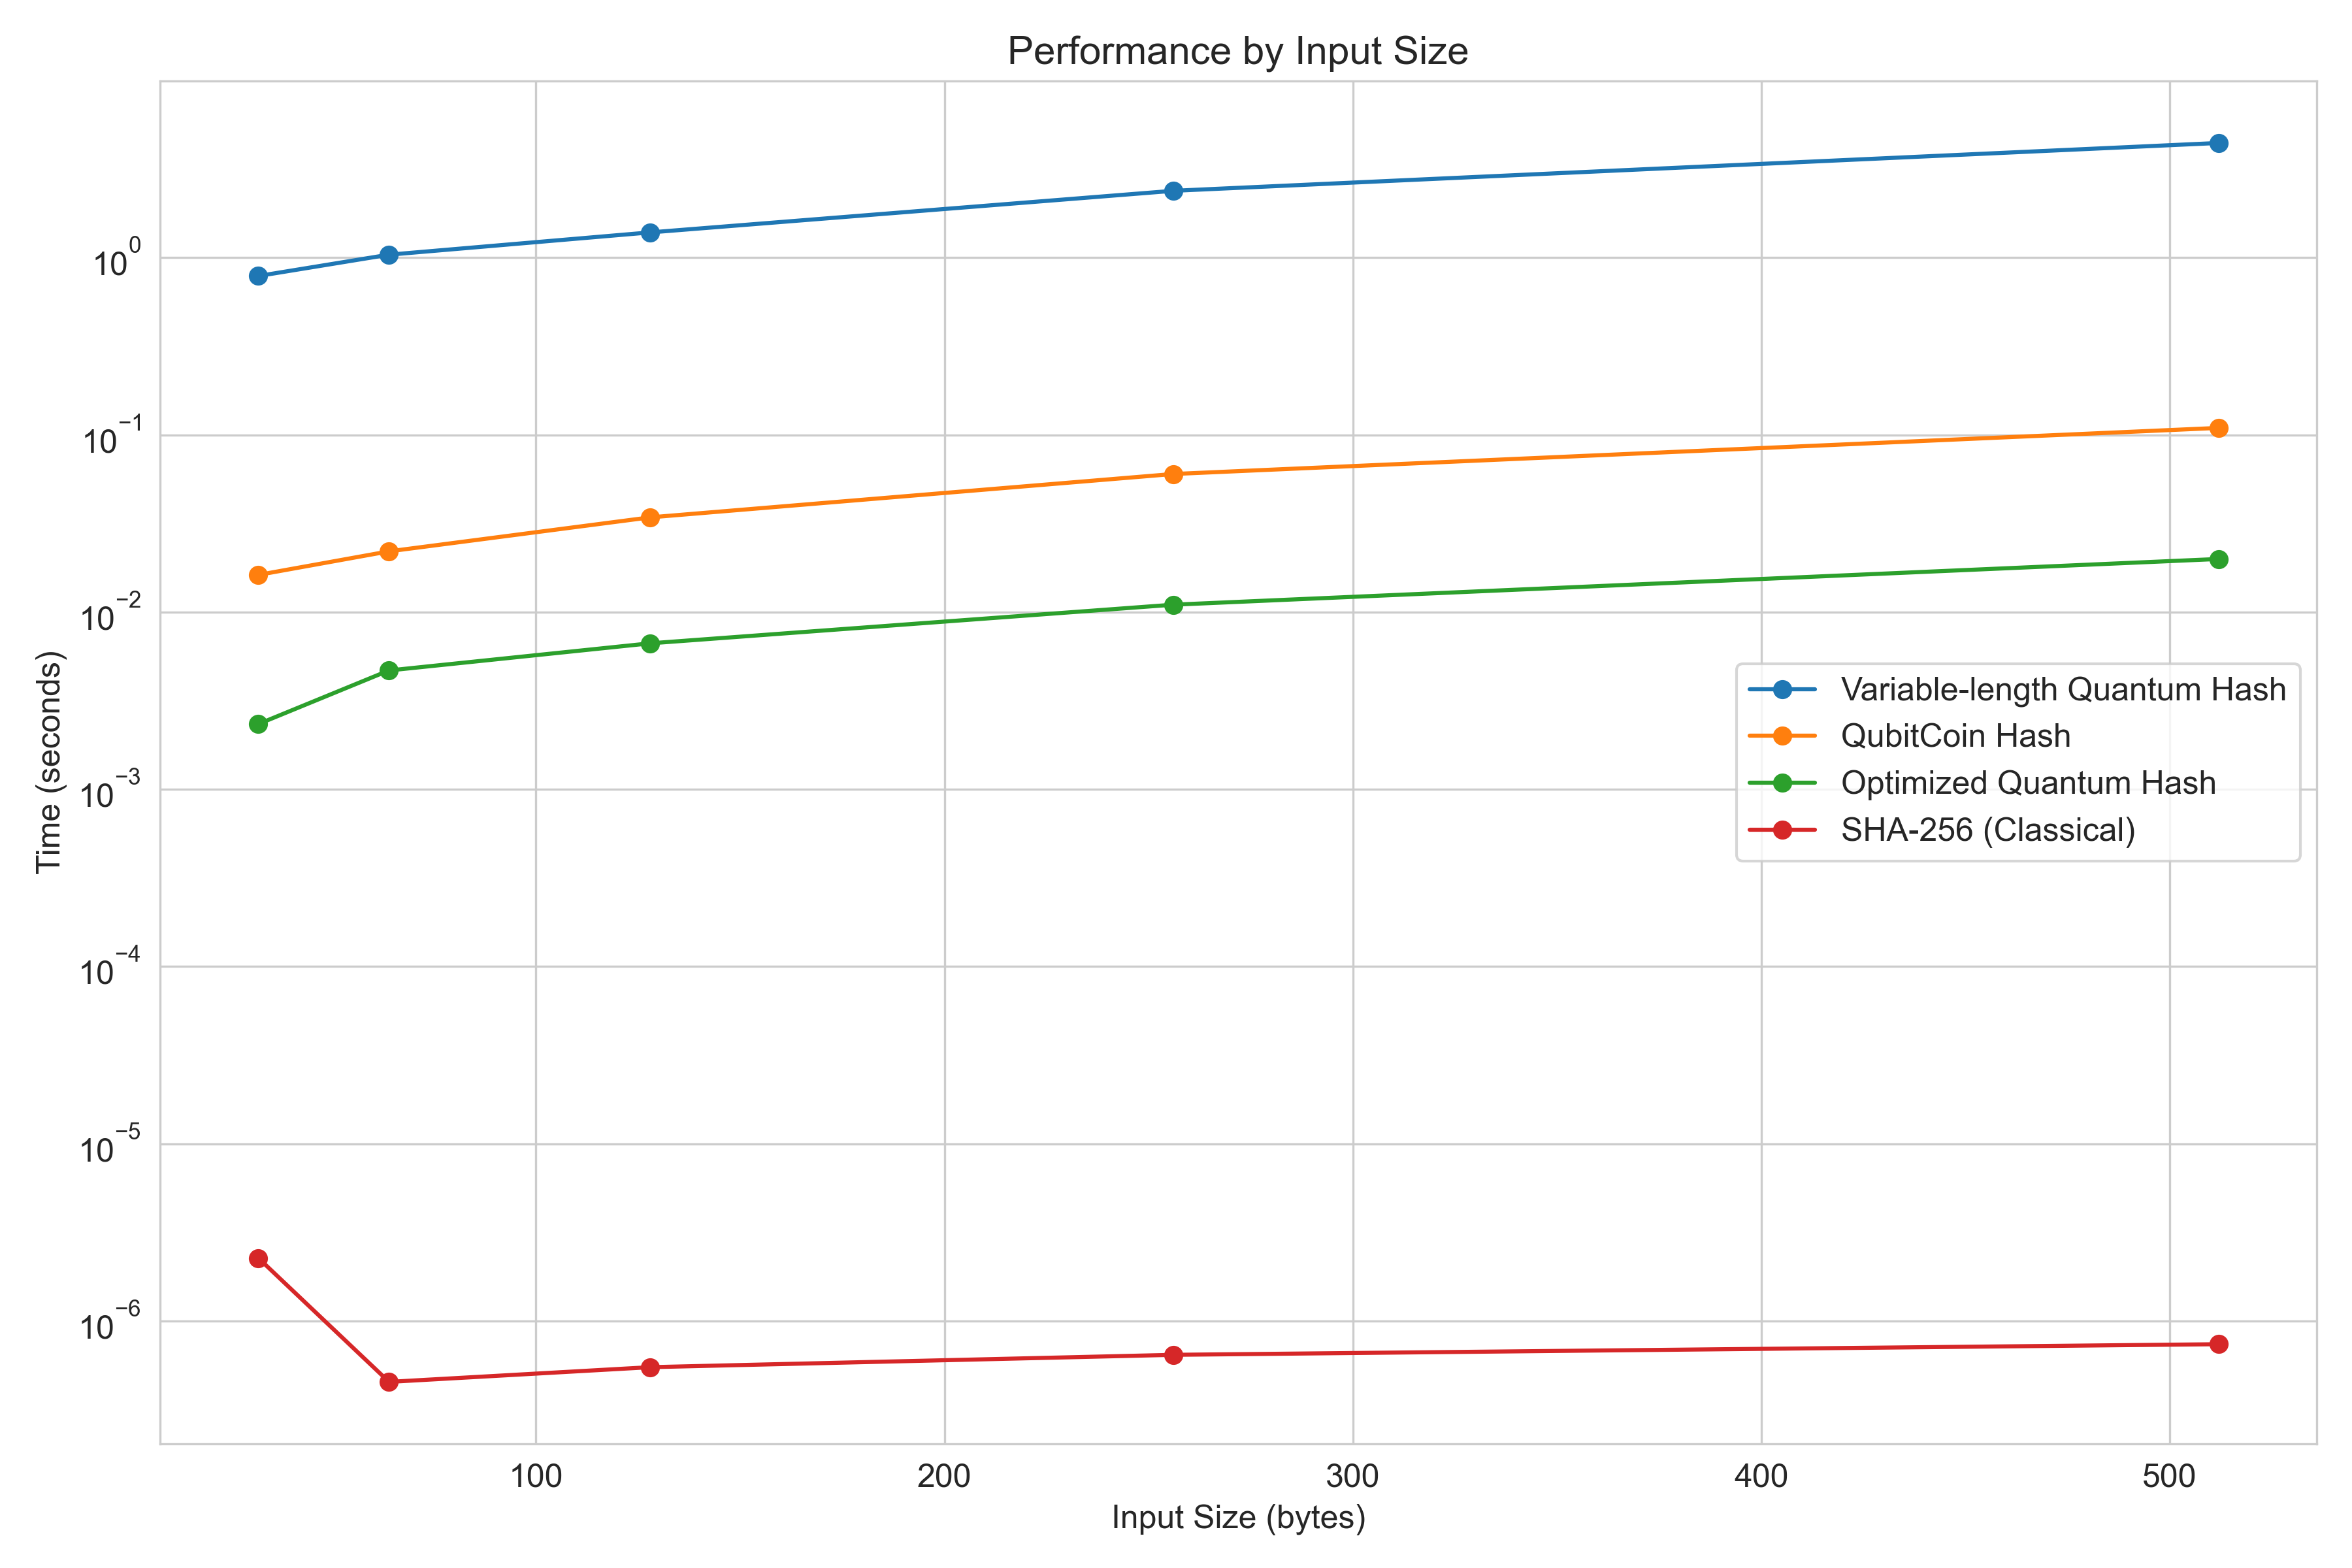
\includegraphics[width=\columnwidth]{visualizations/performance_by_size.png}
\caption{Performance scaling with input size.}
\label{fig:performance_by_size}
\end{figure}

The optimized implementation scales efficiently with input size, maintaining reasonable performance even for larger inputs.

\subsection{Timing Distribution}
Fig. \ref{fig:timing_distribution} shows the distribution of execution times:

\begin{figure}[!ht]
\centering
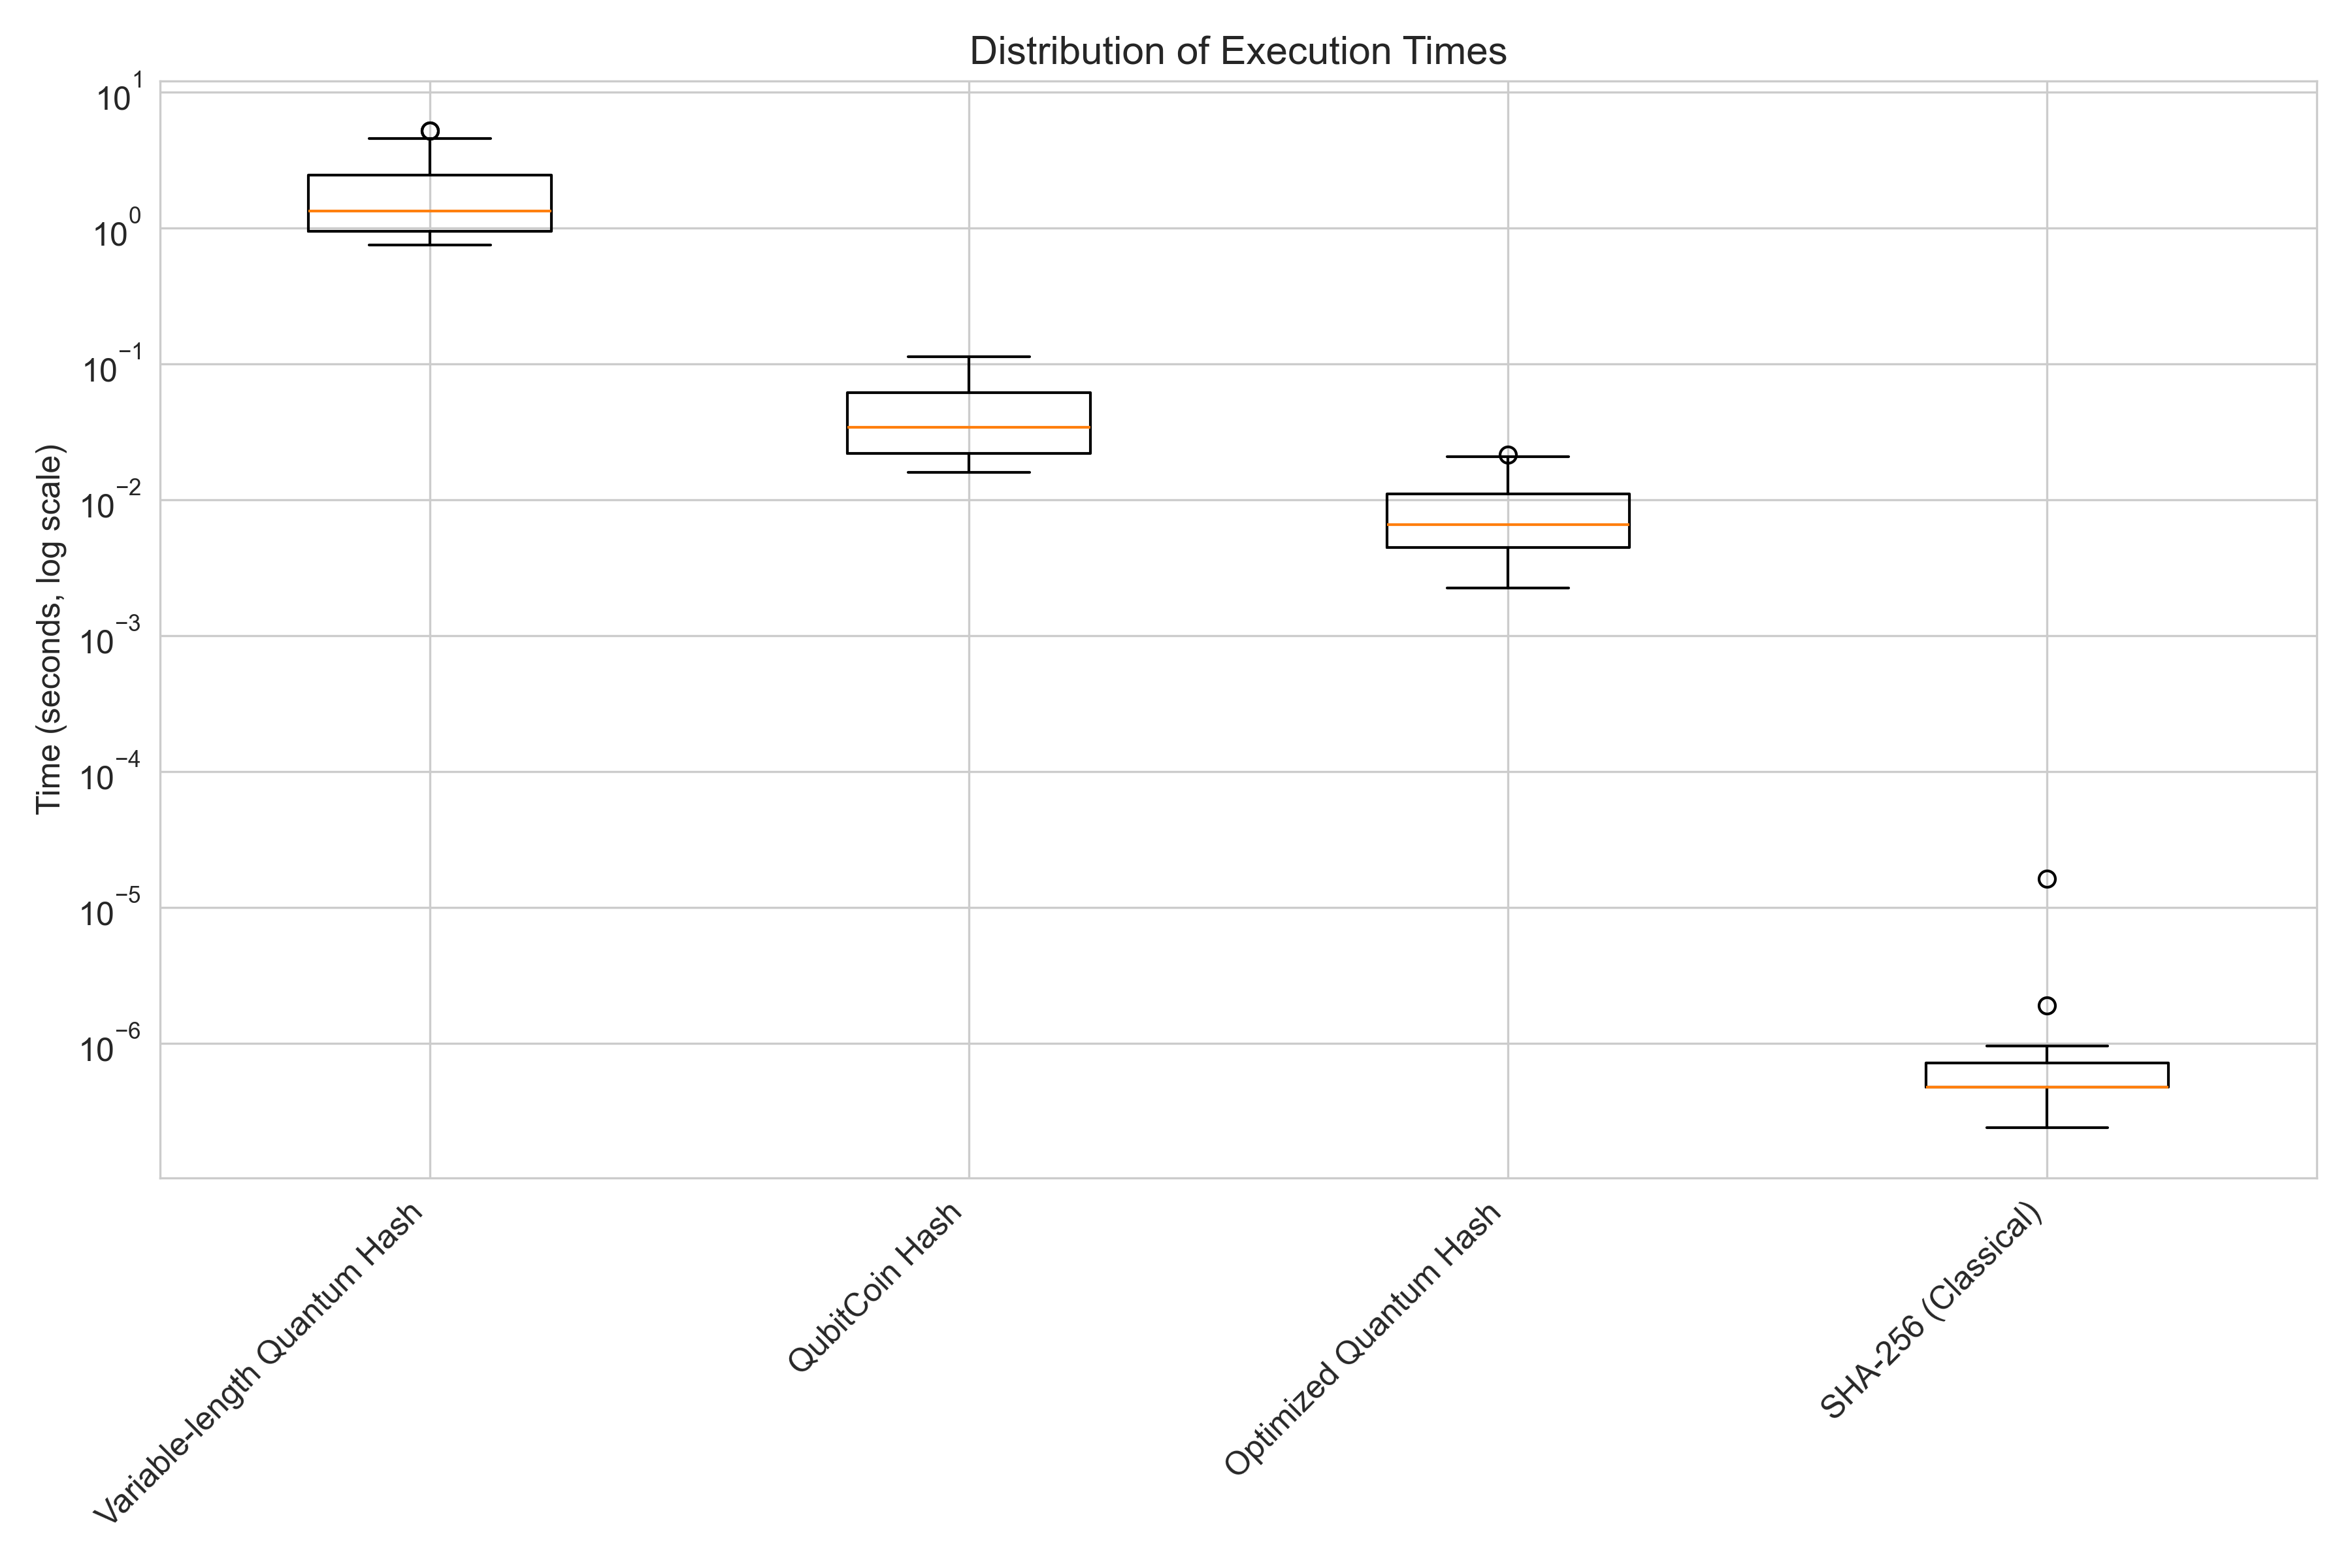
\includegraphics[width=\columnwidth]{visualizations/timing_distribution.png}
\caption{Execution time distribution across hash functions.}
\label{fig:timing_distribution}
\end{figure}

While classical SHA-256 remains significantly faster, our optimized quantum hash is much more practical than previous quantum implementations.

\section{Practical Applications in Blockchain}
Quantum hash functions have several potential applications in blockchain infrastructure during the NISQ era:

\subsection{Quantum-Resistant Proof-of-Work}
Our hash functions could form the basis for quantum-resistant proof-of-work schemes, where miners would need to solve puzzles based on finding inputs that produce hash outputs with specific properties. Since our hash functions provide strong preimage resistance and good avalanche effects, they would create challenging but fair mining puzzles.

\subsection{Hybrid Classical-Quantum Systems}
During the transition to quantum-capable infrastructure, blockchain systems could implement hybrid approaches:
\begin{itemize}
    \item Using quantum hashes for certain high-security operations
    \item Maintaining classical hashes for performance-critical functions
    \item Gradually transitioning as quantum technology matures
\end{itemize}

\subsection{Authenticated Quantum Communication}
Beyond blockchain, our hash functions could enable:
\begin{itemize}
    \item Quantum-secure message authentication codes
    \item Integrity verification for quantum communication
    \item Secure key derivation in post-quantum cryptography
\end{itemize}

\subsection{Performance Considerations}
Implementation in real-world blockchain systems would require:
\begin{itemize}
    \item Optimization for specific quantum hardware architectures
    \item Continued improvements in circuit design and entropy extraction
    \item Balancing security properties with performance requirements
\end{itemize}

\section{Conclusion and Future Work}
We have presented optimized and variable-length quantum hash implementations that significantly improve upon existing approaches like QubitCoin's qHash. Our implementations demonstrate excellent avalanche effects, reasonable entropy, and significantly improved performance, making them viable candidates for integration into quantum-resistant blockchain technologies.

Future work could focus on:
\begin{itemize}
    \item Further optimizing circuit designs for specific quantum hardware
    \item Improving the entropy of the variable-length implementation
    \item Implementing adaptive behaviors to optimize for different input sizes
    \item Developing quantum hash-based signature schemes for blockchain applications
\end{itemize}

As quantum computing continues to mature, hash functions like the ones presented in this paper will play an increasingly important role in ensuring the security and integrity of blockchain systems in a post-quantum world.

\section*{Acknowledgment}
We extend our sincere gratitude to the SuperQuantum YQuantum team for providing this opportunity to participate in such an innovative challenge. Their support and the conceptual framework they provided allowed us to explore the fascinating intersection of quantum computing and blockchain technology.

\end{document}
